% !TEX encoding = UTF-8 Unicode
% !TEX TS-program = xelatex

\documentclass[a4paper,12pt]{article}

\usepackage[pdftex]{graphicx}

\makeatletter
\newcommand\subsubsubsection{\@startsection{paragraph}{4}{\z@}{-2.5ex\@plus -1ex \@minus -.25ex}{1.25ex \@plus .25ex}{\normalfont\normalsize\bfseries}}
\newcommand\subsubsubsubsection{\@startsection{subparagraph}{5}{\z@}{-2.5ex\@plus -1ex \@minus -.25ex}{1.25ex \@plus .25ex}{\normalfont\normalsize\itshape}}
\makeatother
\setcounter{secnumdepth}{5} % how many sectioning levels to assign numbers to
\setcounter{tocdepth}{5} 

\setcounter{topnumber}{3}
\setcounter{bottomnumber}{3}
\setcounter{totalnumber}{5}

\usepackage{listings}
\lstset{
  breaklines=true,
  breakatwhitespace=true,
  columns=fullflexible
}

% !TEX encoding = UTF-8 Unicode
% !TEX root =  main.tex


\usepackage{letter}
\usepackage{colortbl}
\usepackage{soul}
\usepackage{xltxtra} 
\usepackage{xgreek} 
\usepackage{fontspec}
\usepackage{listings}
\usepackage{graphicx}

%
% Tables
\usepackage{colortbl}
\usepackage[table]{xcolor}
\definecolor{lightgray}{gray}{0.9}

%
% Page size
\usepackage[margin=2.5cm]{geometry}
% \setlength{\textheight}{23cm}
% \setlength{\textwidth}{15.5cm}
% \setlength{\oddsidemargin}{0.2cm}
% \setlength{\evensidemargin}{0.2cm}
% \setlength{\topmargin}{-1.2cm}
% %\setlength{\headsep}{1.5cm}
% \setlength{\footskip}{2cm} % space between page number and text

% 1.2 spacing
 \renewcommand{\baselinestretch}{1.1}

%
% Fonts sets
\setmainfont[ItalicFont=cmunsl.ttf,BoldFont=cmunbx.ttf,SmallCapsFont=cmunbx.ttf]{cmunrm.ttf}  
%\setmainfont[Mapping=tex-text]{CMU Serif} 
%\setmainfont[Mapping=tex-text]{Marion} 
%\setmainfont[Mapping=tex-text]{Athelas} 

\setmonofont{Courier New}
%\setmonofont{Tahoma}

\frenchspacing

%
% hyphanation
\hyphenation{
ανα-φο-ρά ατό-μι-κης αρι-θμούς αντι-κει-μέ-νων απα-λοι-φής απρό-σκο-πτης αλγό-ριθ-μοι
αλγό-ριθ-μος απο-τε-λέ-σμα-τα ανα-ζη-τη-θούν αυ-τής αντι-κα-τα-στά-σεις
αντι-κει-με-νο-στρε-φείς αυθ-ύπ-αρ-κτη ανα-πα-ρά-στα-ση αρχι-τε-κτο-νι-κής
ανα-πα-ρά-στα-ση
%
}


%
% Definitions
\newtheorem{definition}{Ορισμός}
\newtheorem{theorem}{Θεώρημα}
\newenvironment{proof}{\noindent{\bf Απόδειξη:}}{\rule[-0.25mm]{0.25cm}{0.25cm}\vspace{1.5ex}}
\newcommand{\proofEnd}{\ \rule[-0.25mm]{0.25cm}{0.25cm}}
\newcommand{\defEnd}{\ \rule[-0.25mm]{0.25cm}{0.25cm}}

%
% Algorithms
\usepackage[figure,vlined,linesnumbered]{algorithm2e}
\SetKwInOut{Input}{Input}
\SetKwInOut{Output}{Output}
\SetKwInOut{Parameter}{Parameter}
\SetKwInput{Algorithm}{Algorithm}
\SetKwInput{Remark}{Remark}
\SetKw{Let}{Let}
\SetKw{Add}{Add}
\SetKwComment{Comment}{{// }}{}

%
% References
% \usepackage[colorlinks,linkcolor=blue,linktocpage]{hyperref}
\usepackage[colorlinks,linkcolor=blue,citecolor=blue,urlcolor=blue,linktocpage]{hyperref}

% Code
\definecolor{customgreen}{rgb}{0,0.6,0}
\definecolor{customgray}{rgb}{0.5,0.5,0.5}
\definecolor{custommauve}{rgb}{0.6,0,0.8}
\lstset{ 
  basicstyle=\small\ttfamily,%,        % the size of the fonts that are used for the code
  breaklines=true,                 % sets automatic line breaking
  commentstyle=\color{customgreen},    % comment style
  firstnumber=1,                % start line enumeration with line 1000
  frame=single,	                   % adds a frame around the code
  keepspaces=true,                 % keeps spaces in text, useful for keeping indentation of code (possibly needs columns=flexible)
  keywordstyle=\color{blue},       % keyword style
  numbers=left,                    % where to put the line-numbers; possible values are (none, left, right)
  numbersep=10pt,                   % how far the line-numbers are from the code
  numberstyle=\tiny\color{customgray}, % the style that is used for the line-numbers
  rulecolor=\color{black},         % if not set, the frame-color may be changed on line-breaks within not-black text (e.g. comments (green here))
  showspaces=false,                % show spaces everywhere adding particular underscores; it overrides 'showstringspaces'
  showstringspaces=false,          % underline spaces within strings only
  showtabs=false,                  % show tabs within strings adding particular underscores
  stepnumber=1,                    % the step between two line-numbers. If it's 1, each line will be numbered
  stringstyle=\color{custommauve},     % string literal style
  tabsize=2,	                   % sets default tabsize to 2 spaces
  aboveskip=-10pt,% 
  belowskip=10pt,%
  title=\lstname                   % show the filename of files included with \lstinputlisting; also try caption instead of title
}

%
% SQL
\lstnewenvironment{SQLcode}{%
\lstset{language=SQL,%
%keywordstyle=\bf\sffamily\color{blue},%
%commentstyle=\color{ForestGreen},%
%stringstyle=\color{Maroon},%
%basicstyle=\ttfamily\normalsize\color{black},%
%frame=lines,%
showspaces=false,% 
showstringspaces=false,%
tabsize=4,% 
%aboveskip=-10pt,% 
%belowskip=10pt,%
lineskip=2pt%
% numbers=left, numberstyle=\tiny, stepnumber=1, numbersep=5pt, numberblanklines=false, %
% breaklines, breakatwhitespace, prebreak=\_, breakindent=0pt %
}}
{}

%
% LaTeX
\lstnewenvironment{latex}{%
\lstset{language=TeX,%
keywordstyle=\bf\sffamily\color{blue},%
commentstyle=\color{ForestGreen},%
stringstyle=\color{Maroon},%
basicstyle=\ttfamily\normalsize\color{black},%
%frame=lines,%
showspaces=false,% 
showstringspaces=false,%
tabsize=4,% 
aboveskip=10pt,% 
belowskip=10pt,%
lineskip=2pt%
% numbers=left, numberstyle=\tiny, stepnumber=1, numbersep=5pt, numberblanklines=false, %
% breaklines, breakatwhitespace, prebreak=\_, breakindent=0pt %
}}
{}


\bibliographystyle{alpha}

\lstdefinestyle{sqlstyle}{
    basicstyle=\ttfamily\small,
    breaklines=true,
    frame=single,
    columns=fullflexible,
    keepspaces=true,
    showstringspaces=false
}

\lstset{style=sqlstyle}

% Ο τίτλος της εργασίας σας
\title{
\normalfont \normalsize 
\textsc{Πανεπιστήμιο Πελοποννήσου\\ 
Θέματα διαχείρισης πληροφοριών και δεδομένων} \\
[10pt] 
\rule{\linewidth}{0.5pt} \\[6pt] 
\huge Μετεωρολογικά Δεδομένα\\
\rule{\linewidth}{2pt}  \\[10pt]
}

% Ο/οι συγγραφείς
\author{Πρίντζιος Θωμάς, Ζερίτης Παντελεήμων}

% Από εδώ και κάτω αρχίζει το κείμενό σας.
\begin{document}

\date{Ιούλιος 2026}

\maketitle

\tableofcontents

\newpage
%
%%
%
\section{Εισαγωγή}\label{sec:introduction}
Σε αυτήν την εργασία θα φτιάξουμε ένα σύστημα συλλογής, αποθήκευσης και δημιουργίας στατιστικών στοιχείων με τις προβλέψεις και τις πραγματικές τιμές από μετεωρολογικά δεδομένα για τις πόλεις Άργος, Τρίπολη, Καλαμάτα, Κόρινθος (Ισθμός), Σπάρτη, Γύθειο, Μεγαλόπολη, Αίγιο, Πύργος (Αμαλιάδα).

Συγκεκριμένα, το σύστημα θα λαμβάνει δεδομένα πρόβλεψης καιρού από τα \texttt{meteo.gr}, \texttt{okairos.gr}, \texttt{emy.gr} και \texttt{openweathermap.org}. Θα συλλέγεται η θερμοκρασία, η υγρασία, ο άνεμος, η βροχόπτωση, η ατμοσφαιρική πίεση και η κατάσταση καιρού και θα αποθηκεύονται σε μια βάση δεδομένων (\texttt{PostgreSQL}), καθώς και τοπικά σε αρχεία \texttt{CSV} για μελλοντική επεξεργασία ή για έλεγχο. Παράλληλα, θα συλλέγονται οι πραγματικές μετρήσεις από μετεωρολογικούς σταθμούς από το \texttt{meteo} και το \texttt{wunderground}, ώστε να υπάρχει σύγκριση μεταξύ πρόβλεψης και πραγματικής κατάστασης σε κάθε πόλη. Με βάση αυτά τα δεδομένα, θа υπολογίζoνται στατιστικά στoιχeίa που δeίχνουν πόσo κoνtά ήtan οι πρoβlέψeιs σtις πρaγμaτiκέs τiμέs.

Τα αποτελέσματα θα παρουσιάζονται με τρόπο ώστε να μπορέσει να απεικονίζεται εύκολα τη συμπεριφορά των προβλέψεων και να εξάγουμε χρήσιμα συμπεράσματα για την αξιοπιστία των μετεωρολογικών δεδομένων.




\section{Σύστημα}\label{sec:res}
Στην ενότητα αυτή παρουσιάζεται η δομή και η λειτουργία του συστήματος για την συλλογή των μετεωρολογικών δεδομένων. Θα παρουσιαστεί η βάση δεδομένων, που αποθηκεύονται οι προβλέψεις και οι πραγματικές μετρήσεις και στην συνέχεια θα αναλυθούν τα αρχεία και οι φάκελοι που βρίσκονται στο σύστημα και το σημείο που εκτελούνται οι μηχανισμοί εξαγωγής δεδομένων (scrapers).

\subsection{Σύνδεση στο σύστημα}\label{sec:connect_to_server}
Για να μπορέσουμε να συνδεθούμε στο σύστημα θα χρειαστεί να ακολουθήσουμε τα παρακάτω βήματα:

\begin{enumerate}
\item 
Συνδεόμαστε στο VPN\footnote{\url{https://digital.uop.gr/sites/default/files/publish/odigies_egkatastasis_vpn.pdf}} του Πανεπιστημίου. 

\item 
Ανοίγουμε το τερματικό εντολών του συστήματος μας και πληκτρολογούμε: 

\begin{lstlisting}
ssh mschin@10.15.29.41
\end{lstlisting}
        
Το \texttt{mschin} είναι το όνομα του χρήστη και \texttt{10.15.29.41} είναι η διεύθυνση (IP) του συστήματος που υπάρχουν οι μηχανισμοί με τα μετεωρολογικά δεδομένα. Οταν συνδεόμαστε στο σύστημα με την παρακάτω εντολή, θα μας εμφανίσει να πληκτρολογήσουμε κωδικό πρόσβασης και θα πληκτρολογήσουμε:

\begin{lstlisting}
meteo#@man0s
\end{lstlisting}

\end{enumerate}

Αν θέλουμε να συνδεθούμε με την εφαρμογή \texttt{Filezilla}, θα πληκτρολογήσουμε τα παραπάνω στοιχεία του συστήματος στην εφαρμογή και θα χρησιμοποιηθεί το port \texttt{22}.

\subsection{Σύνδεση στην βάση δεδομένων}\label{sec:how_to_connect_to_the_database}
Για να μπορέσουμε να εισέλθουμε στην βάση, ανοίγουμε ένα τερματικό, και συνδεόμαστε με την εντολή \texttt{psql -U sensors -h localhost -W}. Το \texttt{sensors} είναι το όνομα της βάσης που θέλουμε να συνδεθούμε και το \texttt{localhost} δείχνει ότι συνδεόμαστε στην τοπική βάση που έχουμε στο σύστημα μας. Στην συνέχεια, θα ζητηθεί κωδικός πρόσβασης, πληκτρολογούμε \texttt{DKM-sensors37}.

Αν θέλουμε να συνδεθούμε ως διαχειριστές, δηλαδή χρησιμοποιώντας το χρήση \texttt{postgres}, ανοίγουμε ένα τερματικό, και συνδεόμαστε με την εντολή 
\begin{lstlisting}
psql -U postgres -h localhost -W 
\end{lstlisting}
Όταν ζητηθεί κωδικός πρόσβασης, πληκτρολογούμε \texttt{meteo\#@man0s}.

Στην Ενότητα~\ref{sec:database_tables} παρουσιάζονται αναλυτικά οι πίνακες που χρησιμοποιούνται στην εργασία και στην Ενότητα~\ref{sec:database_configuration} παρουσιάζονται οι τρόποι δημιουργίας πινάκων.

\subsection{Αρχεία στο σύστημα}\label{sec:directory_structure}
Σε αυτήν την ενότητα θα παρουσιαστεί ο τρόπος που έχουν δομηθεί τα αρχεία στο σύστημα. Η υλοποίηση μας βρίσκεται στον φάκελο με το όνομα \texttt{/meteorological\_data\_new/}. Το αρχείο \texttt{../main/.env} έχει μεταβλητές για τα στοιχεία σύνδεσης της βάσης δεδομένων. Αν θέλουμε να αλλάξουμε το όνομα ή τον κωδικό για να φορτώσουμε την βάση δεδομένων, θα χρειαστεί να τροποποιηθεί το \texttt{.env} αρχείο. Το αρχείο \texttt{/meteorological\_data\_new/scrapy.cfg} είναι το αρχείο ρυθμίσεων της βιβλιοθήκης που χρησιμοποιούμε για τον μηχανισμό εξαγωγής δεδομέων (\texttt{scrapy}). Αυτό το αρχείο είναι απαραίτητο για να τρέξει το \texttt{Scrapy}. Για την τωρινή υλοποίηση, οι μηχανισμοί εξαγωγής δεδομένων (spiders ή αλλιώς scrapers) βρίσκονται στο φάκελο: 

\begin{lstlisting}
meteorological_data_new/main/spiders/
\end{lstlisting}

Οι μηχανισμοί \texttt{meteo\_forecast}, \texttt{okairos\_forecast}, \texttt{emy\_forecast} και \texttt{openweathermap\_forecast} αντλούν προβλέψεις μετεωρολογικών δεδομένων. Για να δούμε τον τον κώδικα από αυτών των μηχανισμών εκτελούμε στο σύστημα:

\begin{lstlisting}
cd ~/meteorological_data_new/main/spiders/
nano meteo_forecast.py
nano okairos_forecast.py
nano emy_forecast.py
nano openweathermap_forecast.py
\end{lstlisting}

Οι μηχανισμοί \texttt{meteo\_live} και \texttt{wunderground\_live} αντλούν τις πραγματικές τιμές που έχουν οι μετεωρολογικοί σταθμοί. Για να δούμε τον κώδικα αυτών των μηχανισμών εκτελούμε στο σύστημα:

\begin{lstlisting}
cd ~/meteorological_data_new/main/spiders/
nano meteo_live.py
nano wunderground_live.py
\end{lstlisting}

Ο φάκελος \texttt{/meteorological\_data\_new/main/data/} περιέχει αρχεία \texttt{CSV} το οποία έχουν τις μετρήσεις που αντλήθηκαν από τις μετεωρολογικές πηγές. Στον φάκελο \texttt{/meteorological\_data\_new/main/logger} υπάρχουν αρχεία καταγραφής ροής του κώδικα (log files) τα οποία καταγραφές για τις επιτυχημένες ή αποτυχημένες διαδικασίες άντλησης δεδομέωνων από τους μηχανισμούς, μαζί με το σφάλμα στην περίπτωση που απέτυχαν. Στον φάκελο \texttt{/meteorological\_data\_new/main/database} υπάρχει το αρχείο \texttt{Python} \texttt{connection.py}, στο οποίο υπάρχει η αρχικοποίηση της βάσης δεδομένων στον κώδικα. Στον φάκελο \texttt{/meteorological\_data\_new/main/preprocessing} υπάρχουν τα αρχεία που κάνουν την προεπεξεργασία των δεδομένων πριν μπούν στην βάση δεδομένων κάνοντας μετρατροπές μονάδων, καθαρισμό δεδομένων κλπ. Πιο συγκεκριμένα, στο αρχείο \texttt{clean.py} υπάρχουν συναρτήσεις καθαρισμού δεδομένων, στο αρχείο \texttt{convert.py} υπάρχουν συναρτήσεις μετατροπής δεδομένων και στο αρχείο \texttt{general.py} υπάρχουν γενικές συναρτήσεις.

Αξίζει να σημειωθεί ότι, στον φάκελο \texttt{dumps} υπάρχουν αποθηκευμένα αρχεία και δεδομένα της βάσης από παλαιότερες υλοποιήσεις. Πιο συγκεκριμένα, ο φάκελος \texttt{old\_2025} περιλαμβάνει αρχεία με κώδικα από παλαιότερες υλοποιήσεις του συστήματος. Αντίστοιχα, ο υποφάκελος \texttt{new\_2026} περιλαμβάνει αρχεία εξαγωγής πινάκων της βάσης δεδομένων που δεν ήταν πλέον απαραίτητοι για την τρέχουσα υλοποίηση. Στον φάκελο \texttt{new\_2026} υπάρχει το \texttt{SQL} αρχείο \texttt{dump\_old\_tables.sql} που περιλαμβάνει όλα τα δεδομένα από τις παλιότερες υλοποιήσεις που ήταν αποθηκευμένες στην βάση δεδομένων. Αυτά έχουν διαγραφτεί από την βάση και τοπικά και υπάρχουν μόνο ως αρχειοθετημένα αρχεία. Αναλυτικότερα, ο πίνακας \texttt{meteodata\_server1\_false} είναι οι προβλέψεις των μετεωρολογικών δεδομένων από το \texttt{meteo.gr} στον πρώτο server που υπήρχε. Ο πίνακας αυτός υπάρχει διότι είχε κάποια λάθη και έτσι δημιουργήθηκε ο πίνακας \texttt{meteodata\_server1\_main} που τα διόρθωνε. Το ίδιο ισχύει και με το \texttt{okairosdata\_server1\_false}, αλλά και με το \texttt{okairosdata\_server1\_main}. Ο πίνακας \texttt{meteodata\_server3} είναι οι προβλέψεις των μετεωρολογικών δεδομένων από το \texttt{meteo.gr} και ο πίνακας \texttt{okairosdata\_server3} είναι για το \texttt{okairos.gr} στον τρίτο server που υπήρχε. Το \texttt{xalazi.gr} δεν χρησιμοποιήθηκε διότι υπήρχε πρόβλημα με τα δεδομένα στο site.


\section{Υλοποίηση}\label{sec:implementation}
Στην ενότητα αυτή παρουσιάζονται πληροφορίες για τους scrapers και για την βάση δεδομένων (\texttt{PostgreSQL}) που χρησιμοποιούνται για την συλλογή, την αποθήκευση των προβλέψεων και των πραγματικών μετεωρολογικών μετρήσεων, αλλά και η δομή των βασικών πινάκων που έχουν δημιουργηθεί. Επιπλέον, περιγράφεται συνοπτικά η διαδικασία εγκατάστασης και ρύθμισης της \texttt{PostgreSQL}\footnote{\url{https://www.postgresql.org/}} και της \texttt{TimescaleDB}\footnote{\url{https://github.com/timescale/timescaledb}} (επέκταση της \texttt{PostgreSQL} για δεδομένα χρονοσειρών), ώστε να είναι περισσότερη αποδοτικά η διαχείριση δεδομένων.

\subsection{Μηχανισμός εξαγωγής δεδομένων (Scrapers)}\label{sec:scrapers}
Για την άντληση μετεωρολογικών δεδομένων θα χρειαστεί να χρησιμοποιήσουμε κάποιο εργαλείο που αντλεί δεδομένα από τις πηγές που παρέχουν μετεωρολογικά δεδομένα. Για να το πετύχουμε, θα χρειαστεί να εγκατασταθεί η \texttt{Python} και το εικονικό περιβάλλον (\texttt{venv - virtual environment}), ώστε να μπορέσουν να εγκατασταθούν και να χρησιμοποιούνται οι απαραίτητες βιβλιοθήκες της εργασίας ανεξάρτητα από τα libraries του συστήματος:

\begin{lstlisting}
sudo apt install python3
sudo apt install python3-venv
\end{lstlisting}

Στη συνέχεια, θα χρησιμοποιηθεί η βιβλιοθήκη \texttt{Scrapy}\footnote{\url{https://www.scrapy.org/}}, η οποία θα ρυθμιστεί ώστε να αντλεί δεδομένα από τις πηγές που απαιτούνται. Το Scrapy είναι ένα πλαίσιο ανάπτυξης λογισμικού της \texttt{Python} για άντληση δεδομένω από ιστοσελίδες. Θα δημιουργήσουμε μηχανισμούς εξαγωγής δεδομένων (scrapers) με το οποίους θα αντλούμε τις προβλέψεις των μετεωρολογικών δεδομένων από τις πηγές \texttt{meteo.gr}, το \texttt{okairos.gr}, το \texttt{emy.gr}, \texttt{openweathermap.org}. Επίσης, Θα δημιουργήσουμε μηχανισμούς με τους οποίους θα αντλούμε μετεωρολογικά δεδομένα από τις μετρήσεις που που διαθέτουν οι σταθμοί τη στιγμή που πραγματοποιείται η διαδικασία συλλογής δεδομένων από τις πηγές \texttt{meteo.gr} και \texttt{wunderground.com}. Στις Ενότητες~\ref{sec:automated_scraper_execution} και ~\ref{sec:manual_scraper_execution} αναλύονται οι τρόποι με τους οποίους μπορούμε να εκτελέσουμε αυτούς τους μηχανισμούς.

\subsection{Βάση δεδομένων}\label{sec:database}
Για την αποθήκευση των μετεωρολογικών δεδομένων, θα χρησιμοποιηθεί η βάση δεδομένων \texttt{PostgreSQL}, καθώς εξυπηρετεί την ανάγκη μας για μία αξιόπιστη, επεκτάσιμη και υψηλής απόδοσης πλατφόρμα. Η εγκατάσταση της PostgreSQL γίνεται μέσω διαχειριστή πακέτων ή από την επίσημη ιστοσελίδα του, ενώ στη συνέχεια προσθέτουμε την επέκταση \texttt{TimescaleDB} για τη διαχείριση δεδομένων χρονοσειρών, κάτι που διευκολύνει τις αναλύσεις δεδομένων με χρονοσφραγίδα και βελτιώνει την αποδοτικότητα της αποθήκευσης.
    
\subsubsection{Εγκατάσταση βάσης δεδομένων}\label{sec:database_installation}
Η πρώτη ενέργεια που έχουμε να κάνουμε είναι να εγκαταστήσουμε την \texttt{PostgreSQL}. Για την εγκατάσταση πληκτρολογούμε στο τερματικό του συστήματος (cmd) \texttt{sudo apt install postgresql postgresql-contrib}. Οταν ολοκληρωθεί η εγκατάσταση, για να επιβεβαιώσουμε ότι λειτουργεί η βάση δεδομένων χωρίς προβλήματα, εκτελούμε την εντολή \texttt{sudo systemctl status postgresql}. Εφόσον η εγκατάσταση έχει πραγματοποιηθεί επιτυχώς και η βάση δεδομένων τρέχει στο σύστημα, στο αποτέλεσμα της εντολής θα πρέπει να εμφανίζεται ότι η κατάσταση της υπηρεσίας είναι \texttt{active (exited)} ή \texttt{active (running)}. Η κατάσταση αυτή επιβεβαιώνει ότι η \texttt{PostgreSQL} έχει ξεκινήσει σωστά και λειτουργεί κανονικά.

\subsubsection{Ρύθμιση βάσης δεδομένων}\label{sec:database_configuration}
Για να ρυθμίσουμε την βάση δεδομένων, θα ανοίξουμε το τερματικό στο σύστημα και θα συνδεθούμε στην βάση μας ως χρήστης \texttt{postgres}, πληκτρολώντας την εντολή \texttt{psql -U postgres}. Αφού συνδεθούμε στην βάση δεδομένων ως χρήστης \texttt{postgres} θα χρησιμοποιήσουμε την εντολή \texttt{\textbackslash password} για να θέσουμε έναν κωδικό για τον χρήστη. Στην συνέχεια, θα μεταβούμε στο αρχείο ρύθμισης της \texttt{PostgreSQL} για να αλλάξουμε ρύθμιση, έτσι ώστε να χρειάζεται η κάθε βάση να κωδικό πρόσβασης για να συνδεθεί ο κάθε χρήστης. Χρησιμοποιούμε την εντολή \lstinline|sudo nano /etc/postgresql/16/main/pg_hba.conf|. Αν εκτελέσουμε σωστά την εντολή θα ανοίξει το αρχείο, θα μεταβούμε στο τέλος του αρχείου και θα εντοπίσουμε τα εξής:

\begin{lstlisting}
local   all             postgres            peer
local   all             all                 peer
\end{lstlisting}

Αφού αποθηκεύσουμε το αρχείο, θα χρειαστεί να επανεκκινήσουμε την υπηρεσία της βάσης δεδομένων ώστε να εφαρμοστούν οι αλλαγές. Αυτό γίνεται με την εντολή \lstinline|sudo systemctl restart postgresql|. Στη συνέχεια, μπορούμε να επαληθεύσουμε ότι η υπηρεσία λειτουργεί κανονικά με την εντολή \lstinline|sudo systemctl status postgresql|.

Μετά την επανεκκίνηση, η σύνδεση στη βάση δεδομένων ως χρήστης \texttt{postgres} θα πραγματοποιείται με την εντολή \lstinline|psql -U postgres -W|, όπου η παράμετρος \texttt{-W} ζητά την εισαγωγή του κωδικού πρόσβασης. Εφόσον η σύνδεση ολοκληρωθεί επιτυχώς, μπορούμε να προχωρήσουμε στη δημιουργία της βάσης δεδομένων που θα χρησιμοποιηθεί από την εφαρμογή.

Αφού ο χρήστης \texttt{sensors} έχει ήδη δημιουργηθεί, το επόμενο βήμα είναι η δημιουργία της βάσης δεδομένων με ιδιοκτήτη τον συγκεκριμένο χρήστη:

\begin{lstlisting}[language=SQL]
CREATE DATABASE sensors OWNER sensors;
\end{lstlisting}

Στη συνέχεια, μπορούμε να συνδεθούμε στη νέα βάση δεδομένων και να ενεργοποιήσουμε την επέκταση \texttt{TimescaleDB}, η οποία είναι απαραίτητη για την αποδοτική διαχείριση χρονοσειρών. Αυτό γίνεται με τις εντολές:

\begin{lstlisting}[language=SQL]
\c sensors
CREATE EXTENSION IF NOT EXISTS timescaledb;
\end{lstlisting}

Με την ολοκλήρωση των παραπάνω βημάτων, η βάση δεδομένων είναι έτοιμη να δεχτεί τους πίνακες και τα μετεωρολογικά δεδομένα της εφαρμογής.


\subsubsection{Πίνακες}\label{sec:database_tables}
Το όνομα της βάσης δεδομένων που χρησιμοποιούμε για την αποθήκευση των μετεωρολογικών δεδομένων είναι η \texttt{sensors}. Στη βάση δεδομένων, ο πίνακας για τις προβλέψεις του \texttt{meteo.gr} είναι ο \texttt{meteodata}. Ο πίνακας για τις προβλέψεις του \texttt{okairos.gr} είναι ο \texttt{okairosdata}. Ο πίνακας για τις προβλέψεις του \texttt{emy.gr} είναι ο \texttt{emydata}. Ο πίνακας για τις προβλέψεις του \texttt{openweathermap.org} είναι ο \texttt{owmdata}. Ο πίνακας για τις τιμές των μετεωρολογικών σταθμών του \texttt{meteo.gr} είναι ο \texttt{meteodata\_live}. Ο πίνακας για τις τιμές των μετεωρολογικών σταθμών του \texttt{wunderground} είναι ο \texttt{wudata\_live}.

Οι πίνακες που αποθηκεύουν δεδομένα με χρονοσειρές μετατρέπονται σε \texttt{hypertables} μέσω της \texttt{TimescaleDB}, με βάση το πεδίο \texttt{timecrawl}. Ένας \texttt{hypertable} αποτελεί ειδική μορφή πίνακα για δεδομένα χρονοσειρών, στην οποία οι εγγραφές χωρίζονται αυτόματα σε μικρότερα χρονικά τμήματα, που ονομάζονται \texttt{chunks}. Με αυτόν τον τρόπο βελτιώνεται η απόδοση τόσο κατά την εισαγωγή νέων μετρήσεων όσο και κατά την εκτέλεση ερωτημάτων που φιλτράρουν δεδομένα με βάση τον χρόνο. Στην Ενότητα~\ref{sec:database_schemas} αναλύονται όλα τα χαρακτηριστικά του κάθε πίνακα που χρησιμοποιείται.


\subsubsection{Σχήματα πινάκων}\label{sec:database_schemas}
Στην ενότητα αυτή παρουσιάζονται τα βασικά σχήματα των πινάκων της βάσης δεδομένων που χρησιμοποιούνται στο σύστημα. Για κάθε πίνακα δίνονται τα πεδία του, οι τύποι δεδομένων, τα βασικά χαρακτηριστικά του και παρατηρήσεις για τον καθένα.

\subsubsubsection{Πίνακας \texttt{meteodata}}

Ο πίνακας \texttt{meteodata} χρησιμοποιείται για την αποθήκευση προβλέψεων μετεωρολογικών δεδομένων του \texttt{meteo} και παρουσιάζονται παρακάτω η αρχικοποιήση του και τα χαρακτηριστικά του:

\begin{lstlisting}[language=SQL, label={lst:meteodata}]
CREATE TABLE meteodata (
    src text,
    city text,
    timecrawl timestamp with time zone NOT NULL,
    day text,
    hour text,
    temperature double precision,
    humidity text,
    wind_km double precision,
    wind_dir text,
    weather_cond text
);

SELECT create_hypertable('meteodata', 'timecrawl');

CREATE INDEX meteodata_timecrawl_idx
ON meteodata (timecrawl DESC);
\end{lstlisting}

\subsubsubsubsection{Περιγραφή πεδίων}
\begin{itemize}
    \item \texttt{src}: η πηγή από την οποία συλλέχθηκαν τα δεδομένα
    \item \texttt{city}: η πόλη στην οποία αντιστοιχεί η μέτρηση
    \item \texttt{timecrawl}: η χρονική στιγμή συλλογής της μέτρησης με ζώνης ώρας (π.χ. GMT+2)
    \item \texttt{day}: η ημέρα της μέτρησης σε μορφή \texttt{DD/MM}, όπου \texttt{DD} είναι η ημέρα και \texttt{MM} ο μήνας
    \item \texttt{hour}: η ώρα της μέτρησης σε μορφή \texttt{HH:MM}, όπου \texttt{HH} είναι η ώρα και \texttt{MM} τα λεπτά
    \item \texttt{temperature}: η τιμή της θερμοκρασίας σε βαθμούς Κελσίου ($^\circ$C)
    \item \texttt{humidity}: η τιμή της σχετικής υγρασίας σε ποσοστό (\%)
    \item \texttt{wind\_km}: η ταχύτητα του ανέμου σε χιλιόμετρα ανά ώρα (km/h)
    \item \texttt{wind\_dir}: η κατεύθυνση του ανέμου, συνήθως σε λεκτική ή συντομογραφική μορφή (π.χ. \texttt{N}, \texttt{NE}, \texttt{SW} ή Β, ΒΑ, ΝΔ)
    \item \texttt{weather\_cond}: η λεκτική περιγραφή των καιρικών συνθηκών
\end{itemize}

\subsubsubsubsection{Παρατηρήσεις}
Το πεδίο \texttt{timecrawl} είναι υποχρεωτικό, καθώς έχει οριστεί ως \texttt{NOT NULL}. Επιπλέον, ο πίνακας μετατρέπεται σε \texttt{hypertable} μέσω της \texttt{TimescaleDB}, με βάση το πεδίο \texttt{timecrawl}, ώστε να υποστηρίζεται αποδοτικότερα η αποθήκευση και η επεξεργασία δεδομένων χρονοσειρών. Τέλος, έχει δημιουργηθεί ευρετήριο στο ίδιο πεδίο με φθίνουσα ταξινόμηση, ώστε να βελτιώνεται η απόδοση σε ερωτήματα που αναζητούν πρόσφατες μετρήσεις.


\subsubsubsection{Πίνακας \texttt{okairosdata}}

Ο πίνακας \texttt{okairosdata} χρησιμοποιείται για την αποθήκευση μετεωρολογικών δεδομένων που προέρχονται από την πηγή \texttt{okairos} και παρουσιάζεται παρακάτω η αρχικοποιήση του και τα χαρακτηριστικά του:

\begin{lstlisting}[language=SQL, label={lst:okairosdata}]
CREATE TABLE okairosdata (
    src text,
    city text,
    timecrawl timestamptz NOT NULL,
    day text,
    hour text,
    weather_cond text,
    temperature double precision,
    wind_km double precision,
    wind_dir text,
    yetos double precision,
    cloudiness text,
    humidity text,
    air_pressure text
);

SELECT create_hypertable('okairosdata', 'timecrawl');

CREATE INDEX okairosdata_timecrawl_idx
ON okairosdata (timecrawl DESC);
\end{lstlisting}

\subsubsubsubsection{Περιγραφή πεδίων}
\begin{itemize}
    \item \texttt{src}: η πηγή από την οποία συλλέχθηκαν τα δεδομένα
    \item \texttt{city}: η πόλη στην οποία αντιστοιχεί η μέτρηση
    \item \texttt{timecrawl}: η χρονική στιγμή συλλογής της μέτρησης με ζώνης ώρας (π.χ. GMT+2)
    \item \texttt{day}: η ημέρα της μέτρησης σε μορφή DD/MM, όπου DD είναι η ημέρα και MM ο μήνας
    \item \texttt{hour}: η ώρα της μέτρησης σε μορφή HH:MM, όπου HH είναι η ώρα και MM τα λεπτά
    \item \texttt{weather\_cond}: η λεκτική περιγραφή των καιρικών συνθηκών
    \item \texttt{temperature}: η τιμή της θερμοκρασίας σε βαθμούς Κελσίου ($^\circ$C)
    \item \texttt{wind\_km}: η ταχύτητα του ανέμου σε χιλιόμετρα ανά ώρα (km/h)
    \item \texttt{wind\_dir}: η κατεύθυνση του ανέμου σε μορφή N, NE, SW ή Β, ΒΑ, ΝΔ
    \item \texttt{yetos}: το ύψος βροχόπτωσης σε χιλιοστά (mm)
    \item \texttt{cloudiness}: η νεφοκάλυψη σε ποσοστό (\%)
    \item \texttt{humidity}: η τιμή της σχετικής υγρασίας σε ποσοστό (\%)
    \item \texttt{air\_pressure}: η τιμή της ατμοσφαιρικής πίεσης σε εκτοπασκάλ (hPa)
\end{itemize}

\subsubsubsubsection{Παρατηρήσεις}
Το πεδίο \texttt{timecrawl} είναι υποχρεωτικό, καθώς έχει οριστεί ως \texttt{NOT NULL}. Επιπλέον, ο πίνακας μετατρέπεται σε \texttt{hypertable} μέσω της \texttt{TimescaleDB}, με βάση το πεδίο \texttt{timecrawl}, ώστε να υποστηρίζεται αποδοτικότερα η αποθήκευση και η επεξεργασία δεδομένων χρονοσειρών. Τέλος, έχει δημιουργηθεί ευρετήριο στο πεδίο \texttt{timecrawl} με φθίνουσα ταξινόμηση, ώστε να βελτιώνεται η απόδοση σε ερωτήματα που αναζητούν τις πιο πρόσφατες εγγραφές.


\subsubsubsection{Πίνακας \texttt{meteodata\_live}}

Ο πίνακας \texttt{meteodata\_live} χρησιμοποιείται για την αποθήκευση ζωντανών μετεωρολογικών δεδομένων που συλλέγονται σε πραγματικό χρόνο από μετεωρολογικούς σταθμούς του \texttt{meteo} και παρουσιάζεται παρακάτω η αρχικοποιήση του και τα χαρακτηριστικά του:

\begin{lstlisting}[language=SQL, label={lst:meteodata_live}]
CREATE TABLE meteodata_live (
    src text,
    city text,
    timecrawl timestamptz NOT NULL,
    day text,
    hour text,
    temperature double precision,
    humidity text,
    wind_km double precision,
    wind_dir text,
    weather_cond text,
    air_pressure double precision,
    yetos double precision
);

SELECT create_hypertable('meteodata_live', 'timecrawl');
\end{lstlisting}

\subsubsubsubsection{Περιγραφή πεδίων}
\begin{itemize}
    \item \texttt{src}: η πηγή από την οποία συλλέχθηκαν τα δεδομένα
    \item \texttt{city}: η πόλη στην οποία αντιστοιχεί η μέτρηση
    \item \texttt{timecrawl}: η χρονική στιγμή συλλογής της μέτρησης με ζώνης ώρας (π.χ. GMT+2)
    \item \texttt{day}: η ημέρα της μέτρησης σε μορφή DD/MM, όπου DD είναι η ημέρα και MM ο μήνας
    \item \texttt{hour}: η ώρα της μέτρησης σε μορφή HH:MM, όπου HH είναι η ώρα και MM τα λεπτά
    \item \texttt{temperature}: η τιμή της θερμοκρασίας σε βαθμούς Κελσίου ($^\circ$C)
    \item \texttt{humidity}: η τιμή της σχετικής υγρασίας σε ποσοστό (\%)
    \item \texttt{wind\_km}: η ταχύτητα του ανέμου σε χιλιόμετρα ανά ώρα (km/h)
    \item \texttt{wind\_dir}: η κατεύθυνση του ανέμου σε μορφή N, NE, SW ή Β, ΒΑ, ΝΔ
    \item \texttt{weather\_cond}: η λεκτική περιγραφή των καιρικών συνθηκών
    \item \texttt{air\_pressure}: η τιμή της ατμοσφαιρικής πίεσης σε εκτοπασκάλ (hPa)
    \item \texttt{yetos}: το ύψος υετού σε χιλιοστά (mm)
\end{itemize}

\subsubsubsubsection{Παρατηρήσεις}
Το πεδίο \texttt{timecrawl} είναι υποχρεωτικό, καθώς έχει οριστεί ως \texttt{NOT NULL}. Επιπλέον, ο πίνακας μετατρέπεται σε \texttt{hypertable} μέσω της \texttt{TimescaleDB}, με βάση το πεδίο \texttt{timecrawl}, ώστε να υποστηρίζεται αποδοτικότερα η αποθήκευση και η επεξεργασία δεδομένων χρονοσειρών.


\subsubsubsection{Πίνακας \texttt{wudata\_live}}

Ο πίνακας \texttt{wudata\_live} χρησιμοποιείται για την αποθήκευση ζωντανών μετεωρολογικών δεδομένων που συλλέγονται σε πραγματικό χρόνο από μετεωρολογικούς σταθμούς του \texttt{wunderground} και παρουσιάζεται παρακάτω η αρχικοποιήση του και τα χαρακτηριστικά του: 

\begin{lstlisting}[language=SQL, label={lst:wudata_live}]
CREATE TABLE wudata_live (
    src text,
    city text,
    timecrawl timestamptz NOT NULL,
    day text,
    hour text,
    temperature double precision,
    humidity text,
    wind_km double precision,
    wind_dir text,
    weather_cond text,
    air_pressure double precision,
    yetos double precision
);

SELECT create_hypertable('wudata_live', 'timecrawl');
\end{lstlisting}

\subsubsubsubsection{Περιγραφή πεδίων}
\begin{itemize}
    \item \texttt{src}: η πηγή από την οποία συλλέχθηκαν τα δεδομένα
    \item \texttt{city}: η πόλη στην οποία αντιστοιχεί η μέτρηση
    \item \texttt{timecrawl}: η χρονική στιγμή συλλογής της μέτρησης με ζώνης ώρας (π.χ. GMT+2)
    \item \texttt{day}: η ημέρα της μέτρησης σε μορφή DD/MM, όπου DD είναι η ημέρα και MM ο μήνας
    \item \texttt{hour}: η ώρα της μέτρησης σε μορφή HH:MM, όπου HH είναι η ώρα και MM τα λεπτά
    \item \texttt{temperature}: η τιμή της θερμοκρασίας σε βαθμούς Κελσίου ($^\circ$C)
    \item \texttt{humidity}: η τιμή της σχετικής υγρασίας σε ποσοστό (\%)
    \item \texttt{wind\_km}: η ταχύτητα του ανέμου σε χιλιόμετρα ανά ώρα (km/h)
    \item \texttt{wind\_dir}: η κατεύθυνση του ανέμου σε μορφή N, NE, SW ή Β, ΒΑ, ΝΔ
    \item \texttt{weather\_cond}: η λεκτική περιγραφή των καιρικών συνθηκών
    \item \texttt{air\_pressure}: η τιμή της ατμοσφαιρικής πίεσης σε εκτοπασκάλ (hPa)
    \item \texttt{yetos}: το ύψος υετού σε χιλιοστά (mm)
\end{itemize}

\subsubsubsubsection{Παρατηρήσεις}
Το πεδίο \texttt{timecrawl} είναι υποχρεωτικό, καθώς έχει οριστεί ως \texttt{NOT NULL}. Επιπλέον, ο πίνακας μετατρέπεται σε \texttt{hypertable} μέσω της \texttt{TimescaleDB}, με βάση το πεδίο \texttt{timecrawl}, ώστε να υποστηρίζεται αποδοτικότερα η αποθήκευση και η επεξεργασία δεδομένων χρονοσειρών.


\subsection{TimescaleDB}\label{sec:timescaledb}

Η \texttt{TimescaleDB} αποτελεί επέκταση της \texttt{PostgreSQL}, η οποία επιτρέπει την αποδοτική αποθήκευση και διαχείριση δεδομένων χρονοσειρών. Ακολουθεί η εγκατάσταση της \texttt{TimescaleDB}\footnote{\url{https://docs.timescale.com/self-hosted/latest/install/installation-linux/}} σε \texttt{Ubuntu}. Τα βήματα εγκατάστασης είναι:

\begin{enumerate}

\item Αρχικά, εγκαθιστούμε τα απαραίτητα πακέτα της \texttt{PostgreSQL} που απαιτούνται για την σωστή λειτουργία της με την εντολή: 

\begin{lstlisting}
sudo apt install gnupg postgresql-common apt-transport-https lsb-release wget
\end{lstlisting}

\item Στη συνέχεια προστίθεται το αποθετήριο της \texttt{TimescaleDB} στο σύστημα με την εντολή:

\begin{lstlisting}
echo "deb https://packagecloud.io/timescale/timescaledb/ubuntu/ $(lsb_release -c -s) main" | sudo tee /etc/apt/sources.list.d/timescaledb.list
\end{lstlisting}

\item Στην συνέχεια εγκαθίσταται το \texttt{TimescaleDB GPG key}, το οποίο χρησιμοποιείται για την επαλήθευση της αυθεντικότητας των πακέτων της \texttt{TimescaleDB} με την εντολή:

\begin{lstlisting}
wget --quiet -O - https://packagecloud.io/timescale/timescaledb/gpgkey sudo gpg --dearmor -o /etc/apt/trusted.gpg.d/timescaledb.gpg
\end{lstlisting}

\item Μετά την προσθήκη της \texttt{TimescaleDB}, γίνεται ενημέρωση της λίστας των πακέτων του συστήματος με την εντολή \texttt{sudo apt update}.

\item Τέλος, πραγματοποιείται η εγκατάσταση της επέκτασης \texttt{TimescaleDB} για την έκδοση \texttt{PostgreSQL 18}:

\begin{lstlisting}
sudo apt install timescaledb-2-postgresql-18
\end{lstlisting}

Μετά την ολοκλήρωση της εγκατάστασης της \texttt{TimescaleDB}, χρειάζεται να ρυθμιστεί στο σύστημα.

\begin{enumerate}

\item Αρχικά εκτελείται το εργαλείο που το ρυθμίζει για να μπορέσει να εκτελεστεί με την εντολή \texttt{sudo timescaledb-tune}. Το εργαλείο αυτό προτείνει τις καλύτερες ρυθμίσεις για παραμέτρους της \texttt{PostgreSQL}, όπως στην ποσότητα χρήση της μνήμης και η διαχείριση των διεργασιών. Μετά την αποδοχή των ρυθμίσεων, οι ρυθμίσεις αποθηκεύονται στο αρχείο της \texttt{PostgreSQL}.

\item Στη συνέχεια, απαιτείται επανεκκίνηση της \texttt{PostgreSQL} ώστε να εφαρμοστούν οι αλλαγές με την εντολή \texttt{sudo systemctl restart postgresql}.

\item Μετά την επανεκκίνηση, θα πραγματοποιηθεί σύνδεση στη βάση δεδομένων με την εντολή \texttt{psql -U postgres}.

\item Τέλος, ενεργοποιείται η επέκταση \texttt{TimescaleDB} μέσα στη βάση δεδομένων με την εντολή \texttt{CREATE EXTENSION IF NOT EXISTS timescaledb;}

\end{enumerate}

Με την ενεργοποίηση της \texttt{TimescaleDB}, η \texttt{PostgreSQL} αποκτά τη δυνατότητα δημιουργίας \texttt{hypertables}, οι οποίες αποτελούν ειδικό τύπο πινάκων που χρειάζονται για την χρήση της \texttt{TimescaleDB}.

\end{enumerate}

Η επιλογή του πακέτου \texttt{timescaledb-2-postgresql-18} έγινε επειδή στο σύστημα χρησιμοποιείται η έκδοση \texttt{PostgreSQL 18}, μετά την αναβάθμιση του cluster από το version \texttt{16} στο \texttt{18}. Είναι σημαντικό η έκδοση της \texttt{TimescaleDB} που εγκαθίσταται να αντιστοιχεί στην έκδοση της \texttt{PostgreSQL} που είναι εγκατεστημένη στο σύστημα.







\section{Εκτέλεση μηχανισμών εξαγωγής δεδομένων}\label{sec:how_to_run}
Σε αυτήν την ενότητα θα αναλυθούν οι τρόποι που μπορούμε να εκτελέσουμε τους μηχανισμούς εξαγωγής μετεωρολογικών δεδομένων αντλώντας μετεωρολογικά δεδομένα. Θα περιγραφτεί η διαδικασία της αυτόματης εκτέλεσης των μηχανισμών αλλά και της χειροκίνητης εκτέλεσης αυτών, με τα βήματα και τις εντολές που απαιτούνται όταν δεν χρησιμοποιείται η αυτόματη εκτέλεση με προγραμματισμένες εργασίες (\texttt{cron jobs}).

\subsection{Αυτόματη εκτέλεση}\label{sec:automated_scraper_execution}
Για να λειτουργεί αυτόματα η συλλογή των δεδομένων, θα χρειαστεί να ρυθμιστούν οι προγραμματισμένες εργασίες στο σύστημα. Για να μπορέσουμε να δούμε τις εργασίες αυτές εκτελούμε στο σύστημα την εντολή \texttt{crontab -e}. Πιο συγκεκριμένα, οι μηχανισμοί εξαγωγής δεδομένων που συλλέγουν τις πραγματικές μετρήσεις από τους σταθμούς εκτελούνται κάθε 20 λεπτά, ώστε να υπάρχoυν καταγραφές των δεδομένων, αφού τα πραγματικά μετεωρολογικά δεδομένα σταθμών αλλάζουν πιο συχνά. Αντίστοιχα, οι μηχανισμοί που συλλέγουν τις προβλέψεις εκτελούνται δύο φορές την ημέρα, στις 09:00 και 22:00. Αυτό γίνεται διότι οι πηγές που αντλούμε τις προβλέψεις ενημέρωνονται 2-3 φορές την μέρα και δεν χρειάζεται να αντλούμε δεδομένα πιο συχνά.

\subsection{Χειροκίνητη εκτέλεση}\label{sec:manual_scraper_execution}
Για να τρέξουμε χειροκίνητα τους μηχανισμούς εξαγωγής δεδομένων, θα χρειαστεί να ανοίξουμε το τερματικό και να μεταφερθούμε στο μέρος της εργασίας. Αυτό θα γίνει με την εντολή \texttt{cd ~/meteorological\_data\_new/main/}. Θα δημιουργήσουμε το εικονικό περιβάλλον για την \texttt{Python} εκτελώντας την εντολή \texttt{python3 -m venv venv}. To ενεργοποιούμε με την εντολή \texttt{source venv/bin/activate} και εγκαθιστούμε τις απαραίτητες βιβλιοθήκες με την εντολή \texttt{pip install -r requirements.txt}. Για την εκτέλεση των μηχανισμών, πηγαίνουμε στον φάκελο της εργασίας. Θα εγκατασταθούν οι βιβλιοθήκες \texttt{scrapy}, \texttt{requests},  \texttt{psycopg2-binary}, \texttt{python-dotenv}, \texttt{PyYAML}, \texttt{matplotlib}, \texttt{pandas}, που είναι σημαντικές για να εκτελεστούν οι μηχανισμοί. Στη συνέχεια, για να τρέξουμε κάποιον μηχανισμό, πηγαίνουμε στον φάκελο με την εντολή \texttt{cd ~/meteorological\_data\_new/main/} και εκτελούμε την εντολή του \texttt{Scrapy} για να εκτελεστούν οι μηχανισμοί:

\begin{lstlisting}
scrapy crawl meteo_forecast
scrapy crawl meteo_live
scrapy crawl okairos_forecast
scrapy crawl wunderground_live
\end{lstlisting}

Αν προσθέσουμε την επιλογή \texttt{-o path/filename.csv} στις εντολές του \texttt{Scrapy} μπορούμε να αποθηκεύσουμε το αποτέλεσμα σε ένα \texttt{CSV} αρχείο. Για παράδειγμα, με την εντολή \texttt{scrapy crawl meteo\_live -o meteo.csv} δημιουργείται και ένα \texttt{CSV} αρχείο στο οποίο καταγράφονται οι μετρήσεις, ώστε να μπορούμε να τις ελέγξουμε και εκτός βάσης δεδομένων.

\section{Στατιστικά}\label{sec:res}
Στην ενότητα αυτή παρουσιάζονται στατιστικά αποτελέσματα που προκύπτουν από τη σύγκριση των μετεωρολογικών προβλέψεων με τις πραγματικές μετρήσεις από σταθμούς. Από τα σχήματα αξιολογείται η ακρίβεια των προβλέψεων ως προς την θερμοκρασία, για διαφορετικές πόλεις και χρονικές περιόδους. Παρόλο που το σύστημα επιτρέπει την εξαγωγή πολλών στατιστικών διαγραμμάτων, στην εργασία παρουσιάζονται συγκεκριμένα παραδείγματα, ώστε να γίνει πιο κατανοητή η αξιολόγηση των δεδομένων. Στον φάκελο του συστήματος υπάρχει αρχείο \texttt{python} το οποίο δημιούργησε τα σχήματα~\ref{fig:tripoli-temp-25-01} και~\ref{fig:tripoli-meteo-2501}. Για να εκτελεστεί πηγαίνουμε στο σημείο του αρχείου με την εντολή \texttt{cd ~/meteorological\_data\_new/main/statistics/} και εκτελούμε το αρχείο \texttt{python3 meteo.py}.

Στο Σχήμα~\ref{fig:tripoli-temp-25-01} απεικονίζεται τη σύγκριση των προβλέψεων θερμοκρασίας από τις πηγές \texttt{meteo.gr} και \texttt{okairos.gr} με τις πραγματικές μετρήσεις από τους σταθμούς \texttt{meteo (live)} και \texttt{wunderground (live)} για την Τρίπολη σε διάστημα 24 ωρών για την ημερομηνία 25/1. Παρατηρείται ότι και οι δύο προβλέψεις δείχνουν να έχουν μία γενική τάση της θερμοκρασίας μέσα στη μέρα, όμως υπάρχουν αποκλίσεις κυρίως τις πρωινές ώρες και το βράδυ. Οι πραγματικές μετρήσεις εμφανίζουν μεγαλύτερες μεταβολές, ενώ οι προβλέψεις είναι πιο ομαλές. Συνολικά, οι προβλέψεις φαίνεται να προσεγγίζουν σωστότερα τη θερμοκρασία με μικρές διαφορές.

\begin{figure}[tb]
      \centering
      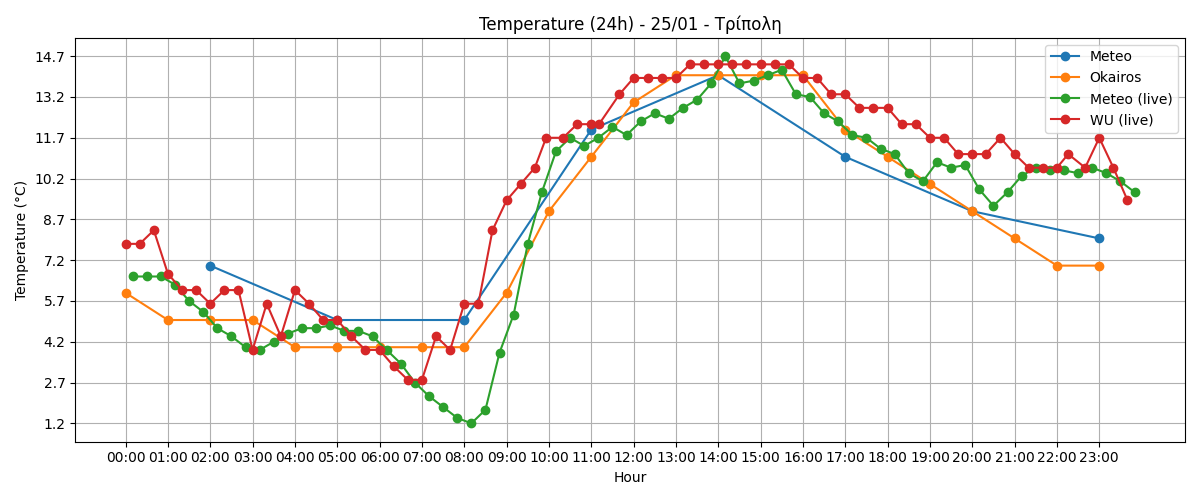
\includegraphics[width=0.9\linewidth]{photos/plot_25_01_2026_24h.png}
      \caption{Σύγκριση προβλέψεων και πραγματικών μετρήσεων θερμοκρασίας όλων των πηγών για την Τρίπολη (25/01)}
      \label{fig:tripoli-temp-25-01}
\end{figure}

Το Σχήμα~\ref{fig:tripoli-meteo-2501} παρουσιάζεται η πρόβλεψη θερμοκρασίας από το \texttt{meteo.gr} σε σύγκριση με τις πραγματικές μετρήσεις (live) για την Τρίπολη στις 25/01. Η πρόβλεψη ακολουθεί την ημερήσια τάση της θερμοκρασίας, με άνοδο μέχρι το μεσημέρι και πτώση της προς το βράδυ. Παρατηρούνται διαφορές κυρίως τις πρώτες πρωινές ώρες, όπου οι πραγματικές τιμές είναι χαμηλότερες από τις προβλεπόμενες. Συνολικά, η πρόβλεψη δίνει μια καλή εικόνα της πορείας της θερμοκρασίας μέσα στην ημέρα, αλλά δεν αποτυπώνει πλήρως τις μικρές διακυμάνσεις των πραγματικών μετρήσεων.

\begin{figure}[h]
      \centering
      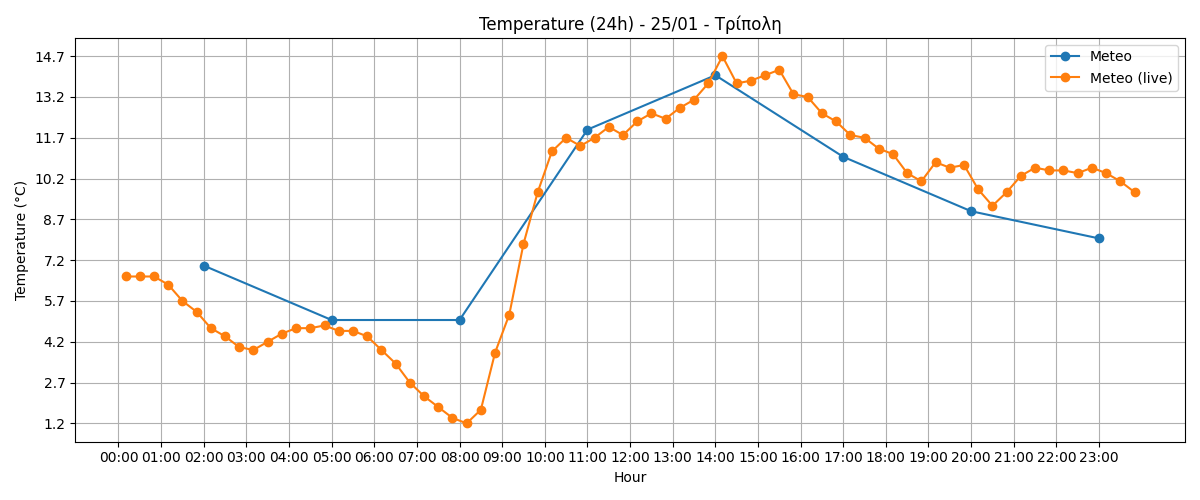
\includegraphics[width=0.9\linewidth]{photos/meteo_25_01_2026_24h.png}
      \caption{Σύγκριση πρόβλεψης και πραγματικών τιμών  θερμοκρασίας του meteo.gr για την Τρίπολη (25/01)}
      \label{fig:tripoli-meteo-2501}
\end{figure}

% \bibliography{sample}
\end{document}
